\documentclass{llncs}
\RequirePackage[english]{babel} % Se fizerem o texto em ingles
\usepackage[english]{babel}   
\usepackage[latin1]{inputenc}
%\usepackage[utf8x]{inputenc}
\usepackage[T1]{fontenc}

\usepackage[fleqn]{amsmath}
\usepackage{amssymb}
\usepackage{makeidx}  % allows for indexgeneration
\usepackage{graphicx}  % allows for indexgeneration
\usepackage{subfig}  % allows for indexgeneration
\usepackage{color}  % allows for indexgeneration
\usepackage{url}
\usepackage{hyperref}
\usepackage{float}
\usepackage{mathtools}
\usepackage{acronym}
\newacro{API}{Application Programming Interface}
\newacro{AES}{Advanced Encryption Standard}
\newacro{BOSH}{Bidirectional-streams Over Synchronous HTTP}
\newacro{CBC}{Cipher Block Chaining}
\newacro{CSS}{Cascading Style Sheets}
\newacro{CPU}{Central Processing Unit}
\newacro{CRUD}{Create, Read, Update and Delete}
\newacro{DOM}{Document Object Model}
\newacro{DTLS}{Datagram Transport Layer Security}
\newacro{FMS}{Flash Media Server}
\newacro{HTML}{HyperText Markup Language}
\newacro{HTTP}{Hypertext Transfer Protocol}
\newacro{ICE}{Interactive Connectivity Establishment}
\newacro{IPv4}{Internet Protocol Version 4}
\newacro{IPv6}{Internet Protocol Version 6}
\newacro{IP}{Internet Protocol}
\newacro{MPEG}{Moving Picture Experts Group}
\newacro{NAT}{Network Address Translation}
\newacro{P2P}{Peer-to-peer}
\newacro{PSTN}{Public Switched Telephone Network}
\newacro{RTMP}{Real Time Messaging Protocol}
\newacro{RTMFP}{Real-Time Media Flow Protocol}
\newacro{RFC}{Request For Comments}
\newacro{SAMI}{Synchronized Accessible Media Interchange}
\newacro{SCTP}{Stream Control Transmission Protocol}
\newacro{SRTP}{Secure Real-time Transport Protocol}
\newacro{RTCP}{Real Time Control Protocol}
\newacro{SRTCP}{Secure RTCP}
\newacro{RTP}{Real-time Transport Protocol}
\newacro{SDP}{Session Description Protocol}
\newacro{SIP}{Session Initiation Protocol}
\newacro{SIMPLE}{SIP for Instant Messaging and Presence Leveraging Extensions}
\newacro{SMIL}{Synchronized Multimedia Integration Language}
\newacro{SMS}{Short Message Service}
\newacro{SRT}{SubRip Text}
\newacro{STUN}{Session Traversal Utilities for NAT}
\newacro{SVG}{Scalable Vector Graphics}
\newacro{TCP}{Transmission Control Protocol}
\newacro{TLS}{Transport Layer Security}
\newacro{TMN}{This Means Nothing}
\newacro{TURN}{Traversal Using Relays around NAT}
\newacro{UDP}{User Datagram Protocol}
\newacro{VoIP}{Voice Over IP}
\newacro{WebRTC}{Web Real-Time Communication}
\newacro{WebVTT}{Web Video Text Tracks}
\newacro{XAML}{eXtensible Application Markup Language}
\newacro{XEP}{XMPP Extensions}
\newacro{XML}{eXtensible Markup Language}
\newacro{XMPP}{Extensible Messaging and Presence Protocol}
\newacro{XHTML}{eXtensible Hypertext Markup Language}
\overfullrule=2cm


\begin{document}
\pagestyle{plain}
\mainmatter              % start of the contributions

\title{Comunica��es Hiperligadas: Novo Paradigma de Comunica��o e Colabora��o, potenciado pela Tecnologia WebRTC}
\author{%
	Henrique Lopes Rocha \\
	email1: henrique.rocha@ist.utl.pt \\
}
\institute{Instituto Superior T�cnico}

\maketitle              % typeset the title of the contribution

\begin{abstract}
    In here put your abstract. Sed ut perspiciatis unde omnis iste natus error sit voluptatem accusantium doloremque laudantium, totam rem aperiam, eaque ipsa quae ab illo inventore veritatis et quasi architecto beatae vitae dicta sunt explicabo. Nemo enim ipsam voluptatem quia voluptas sit aspernatur aut odit aut fugit, sed quia consequuntur magni dolores eos qui ratione voluptatem sequi nesciunt. Neque porro quisquam est, qui dolorem ipsum quia dolor sit amet, consectetur, adipisci velit, sed quia non numquam eius modi tempora incidunt ut labore et dolore magnam aliquam quaerat voluptatem. 
\keywords{keyworkd1, keyworkd2, keyworkd3}
\end{abstract}

\section{Introduction}
  The need to build a global communications network in an age when almost nobody had access to technology and the number of future users was unpredictable, caused that some protocols weren't suitable for a huge increase on the amount of publicly known users. \ac{IPv4} limits the number of public addresses in such a way that today is scarce \cite{ipv4}. One way to overcome this problem was the development of a mechanism that groups multiple address into a single one, the machine that is assigned that address is then responsible to redirect messages to members of its group through their private addresses, each member of the private network is identified publicly by the same \ac{IP} address with a different port, this technique is also known as \ac{NAT}.

Initially \ac{NAT} offered an alternative to address exhaustion and a minimal sensation of security. There are four types of \ac{NAT} implementations\footnote{rfc3489}, \textit{Full Cone NAT}, \textit{Restricted Cone NAT}, \textit{Port Restricted Cone NAT}, \textit{Symmetric NAT}.

\textit{Full Cone} \ac{NAT} maps public each \ac{IP} address and port to a private \ac{IP} address and port, any external host can communicate with private hosts through their mapped public address and port. This represents the least restrictive type of \ac{NAT} and as we will later, the unique type of \ac{NAT} that enables real time communications from point to point.

\textit{Restricted Cone} \ac{NAT} requires that a private client must first send a message to an external host before it can receive messages from the same host. With this type of \ac{NAT}, the private client can be contacted from any port of the same external host.

\textit{Port Restricted Cone} \ac{NAT} works in the same way as Restricted Cone \ac{NAT}, but it only allows communications from the same external host's IP address and port, ignoring all messages from other applications within the same external host.

\textit{Symmetric} NAT maps different ports for each connection, as we will see later, this type of \ac{NAT} represents a problem on real time communications.

\textit{Asymmetric} \ac{NAT} became a vulgar configuration on the web. As a direct result, problems started to appear, the amount of ports that \ac{IP} makes available is also small compared to our current needs, worse than that, \ac{NAT} also difficult end-to-end communication, forcing most of applications that follow this model to be implemented ineffectively.

Applications based on multimedia and file sharing have been one of the most strained by \ac{NAT}. Those kind applications require real time communication in order to achieve the best performance. \ac{STUN} and \ac{TURN} \cite{natvoip} servers are a possible solution to overpass \ac{NAT}, although, none of those can establish direct connections on multiple level \ac{NAT}s.

\ac{STUN} servers are quite simple, they receive requests from \ac{NAT}ed clients, the source address of a request is the public address that \ac{NAT} mapped to the client, \ac{STUN} servers will then reply the mapped public address to the client, so it knows its associated public \ac{IP} address and port. Symmetric \ac{NAT} changes \ac{IP} port for each different connection, for that reason \ac{STUN} servers will reply the \ac{IP} address and port of their connection, which will be useless to clients connections, that's why Symmetric \ac{NAT} represents a problem for real time communications.   

On the other hand, \ac{TURN} uses public servers to redirect traffic between private endpoints, it may use a \ac{P2P} network relay to find the best peer, but after that the behavior is much like client-server. Direct communication is only achieved by \ac{STUN} when \ac{NAT} is a type \textit{full cone}. \ac{ICE} uses \ac{STUN} when it's possible and \ac{TURN} otherwise.

Most of client-server applications aren't affected by \ac{NAT} when the servers are public, but they're inadequate for real time communication between two private endpoints. Clearly this type of communication requires a more expensive infrastructure and, in most cases, more network usage, leading to a worse quality of service. The requirements of video communication makes this kind of model unsuitable.

When connection is established, either in a direct or indirect way (via \ac{TURN} servers), \ac{WebRTC} came to simplify how audio and video are transmitted through web browsers.

\ac{WebRTC} is an open source technology that defines a collection of standard protocols and JavaScript \ac{API}s for web browser real time communications without installing any additional application or plug-in.

\begin{figure}[H]
	\begin{center}
		\centering
		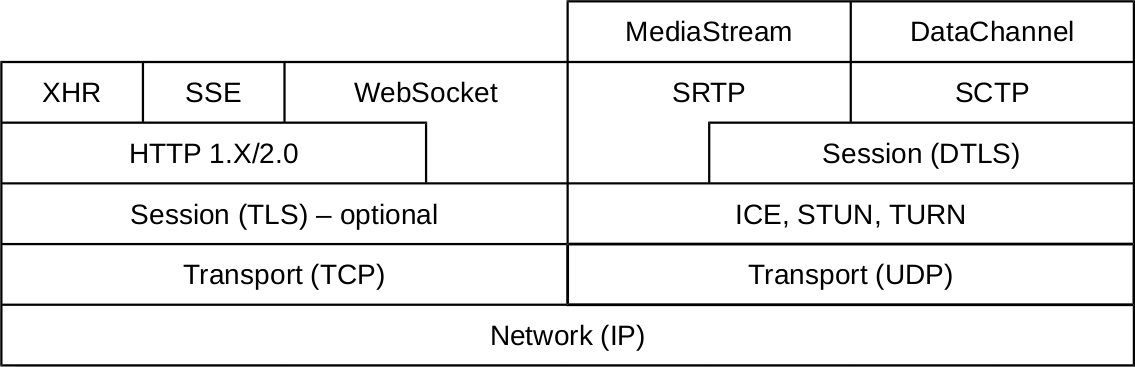
\includegraphics[width=0.9\textwidth]{figures/webrtc_stack.png}

	\caption{WebRTC protocol Stack}
	\end{center}
\end{figure}

\ac{WebRTC} defines three main \ac{API}s: GetUserMedia, PeerConnection and DataChannel. 

\begin{itemize}
  \item \textbf{GetUserMedia} allows from the browser to access to camera, microphone and device screen. 

  \item \textbf{PeerConnection} aquires connection data and negotiates with peers.

  \item \textbf{DataChannel} allows to send whatever type of data to other peers.
\end{itemize}

\ac{WebRTC} uses \ac{UDP} for transporting data, which provides lower latencies than \ac{TCP}, but is not reliable and packet order and integrity are not assured. \ac{SCTP} and \ac{SRTP} are used for streaming data, providing a mechanism for congestion control and partial reliable delivery over \ac{UDP}. All transferred audio, data and video must be encrypted with \ac{DTLS} which provides the same security guarantees as \ac{TLS}. 

\ac{TLS} doesn't support independent record decryption, for that it requires a reliable transport channel, typically \ac{TCP}. The decryption of a record depends on the previous record, which for unreliable transport protocols like \ac{UDP} may represent a problem, either due to packet loss or different reception order.

\ac{DTLS} is similar to \ac{TLS}, but on top of \ac{UDP}, the main difference is the inclusion of a sequence number per packet that is used for packet re-ordering on reception and protects from duplicated packets. If a packet sequence number is less than the expected sequence number the packet is discarded. If a packet sequence number is greater than the expected sequence number the packet may be enqueued or discarded. By knowing the sequence of messages that are sent and received in \ac{TLS}, timers are used for packet retransmission avoiding acknowledgement messages.

\ac{WebRTC}'s \textit{Data Channel} is built on top of \ac{SCTP}, which is secured by \ac{DTLS}. A \textit{Data Channel} has one incoming stream and one outgoing stream, providing bidirectional communication. Each data channel direction can be tweaked for reliable or unreliable transmission, the same can be done for order delivery. A priority can also be defined for improving the quality of service for a particular stream compared to another.

\textit{Skype}\footnote{skype's site} is an application that allows video, voice and instant messaging communication over proprietary protocols, its main strength is the amount of users that are using it nowadays. But compared to \textit{Skype}, \ac{WebRTC} applications don't need to be pre-installed.

\textit{Google Hangouts}\footnote{Hangouts site} is a video conference web application, in the past in order to use \textit{hangouts} on a web browser a plug-in was needed to be installed, nowadays hangouts is using \ac{WebRTC}.

Jitsi Meet\footnote{jitsi meet} is a \ac{WebRTC} collaborative application that uses Jitsi Videobridge for high quality and scalable video conferences and supports shared document editing. Jitsi Videobridge is a server that enables multiparty video calls.





\section{\color{red}Signaling}
  \subsection{Signaling, meet and get to know}


  Signaling is the most important process for applications to exchange connection information about peers and servers, their capabilities and meta-data.

  \ac{WebRTC} doesn't implement signaling, different applications may require different protocols, there is no single answer that fits all problems. Amongst multiple options, signaling can be done by using \ac{SIP}, \ac{XMPP}, \emph{WebSockets}, \emph{Socket.io} or by implementing a custom protocol.

  \ac{WebRTC} uses \ac{SDP} \cite{rfc4566} to define peer connection properties such as types of supported media, codecs, protocols used and network information. An \ac{SDP} offer describes to other peers the expected type of communication and its details, such as used transport protocols, codecs, security and other.

  One of signaling requisites is bi-directional communication over \ac{HTTP}. \ac{HTTP} works on a request followed by a server response, by other words, follows a unidirectional communication. Sometimes it's required that some informations are obtained in real time, as we saw, some \ac{NAT}'s don't support callbacks from servers, one technique to overcome this problem is polling.

  Polling consists on sending periodic messages that the server responds immediately with empty content or fresh information. Real time communications are unpredictable, if the time between periodic requests is short, most of the time the server will return empty results wasting network bandwidth and energy. On the other hand, if the time between periodic requests is large, newer messages may arrive later.

  A technique called long polling consists on making the server hold the request until there is fresh information or expiring after some time, after the message receipt, the client makes another request. Long polling technique results on a better network usage and a faster server response, but both simple polling and long polling requests are sent with \ac{HTTP} headers, which adds data overhead, especially for short messages.

  The WebSocket protocol \cite{rfc6455} provides bidirectional communications over a full-duplex socket channel. WebSocket handshake phase specifies an \ac{HTTP} header in order to upgrade to \emph{WebSocket} type of communication, the remainder messages are done without \ac{HTTP} headers, which leads to much smaller messages and better network usage. WebSockets may not be available on every web browser, frameworks like \emph{socket.io}\footnote{\url{http://socket.io/}} and \emph{SockJS}\footnote{\url{http://github.com/sockjs}} uses \ac{HTTP} when there is no support for WebSockets. 

  \ac{BOSH}\cite{xep0124} is a technique based on long polling that uses two socket connections and allow sending client messages to server while a previous request is held.

  \ac{BOSH} specification assumes that a connection manager is implemented to handle \ac{HTTP} connections. This connection manager is basically a translator from \ac{HTTP} to raw message so the server may think this communication is performed over \ac{TCP}.

  When the connection manager holds for a response for too long it responds with an empty body, this technique prevents an \ac{HTTP} session from expiring when the client is waiting for a response, thus expanding the session time. Expiring sessions can be expensive due to the overhead of establishing new connections, it worsens even more when \ac{HTTP} is used over \ac{SSL}.

  If the server is holding a request, it maintains a second connection to receive more requests from the same client. The request on hold returns immediately with a possible empty body leaving its socket free, while the second connection serves the polling loop. The exchange of roles of those two connections allow to pull data from multiple contexts instead of being locked in just one.

  If the client has data to send while a request is still open, it establishes a second socket connection to the connection manager to send a new request. The connection manager immediately responds to the previously held request (possibly with no data) and holds open this new request. This results in the connections switching roles.

  \ac{SIP} \cite{rfc3261} is protocol used for negotiation, creation, modification and finalization of communication sessions between users. \ac{SIP} follows a client/server architecture with \ac{HTTP} like messages and it can be used as signaling protocol. The advantage of \ac{SIP} is the ability to make video and voice call's applications over \ac{IP} networks.

  The working group \ac{SIMPLE}\footnote{\url{https://datatracker.ietf.org/wg/simple/documents/}} proposed the creation of \ac{SIP} extensions, namely presence information \cite{rfc5263} and instant messaging \cite{rfc3428}.

  \ac{SIP} is used in \ac{VoIP} applications due to its compatibility with \ac{PSTN}. Service providers making their \ac{SIP} infrastructures available through WebSockets. Frameworks like \emph{jsSIP}\footnote{\url{http://jssip.net/}}, \emph{QoffeeSIP}\footnote{\url{http://qoffeesip.quobis.com/}} and \emph{sipML5}\footnote{\url{http://sipml5.org/}} are used on client side to parse and encode \ac{SIP} messages, making \ac{SIP} accessible to web based applications. 

  \ac{SIP} with \emph{WebSockets} can be used as a signaling method for \ac{WebRTC} applications, it allows web browsers to have audio, video and \ac{SMS} capabilities like mobile phones. For instance, it's possible to inter-operate web communications with \ac{SIP} networks, mobile and fixed phones.

  \ac{XMPP} was initially developed for instant messaging and presence (Jabber\footnote{\url{http://jabber.org/}}). It is nowadays an open technology for standardized, decentralized, secure and extensible real-time communications. 

  \ac{XMPP} messages are \ac{XML} based, which are attractive for applications that need structured messages and rich hypermedia. \ac{XMPP} advantage is the addition of extensions, for example \cite{xep0096}, which adds file transfer capabilities between two entities and \cite{xep0045} which enables multi-user chat.

  \ac{XMPP}'s bi-directional communication is achieved through \ac{BOSH} \cite{xep0206}, which basically consists on long polling. This kind of communication is also possible through WebSockets \cite{rfc7395}.

  Amongst multiple XMPP server solutions are: \emph{ejabberd}\footnote{\url{http://jabberd.im/}}, \emph{Metronome}\footnote{\url{http://lightwitch.org/metronome}}, \emph{Openfire}\footnote{\url{http://igniterealtime.org/projects/openfire/}} and \emph{Prosody}\footnote{\url{http://prosody.im/}}. \emph{Ejabberd} is the one that implements more \ac{RFC} specifications and \ac{XEP}s\footnote{\url{http://en.wikipedia.org/wiki/Comparison_of_XMPP_server_software}}.

  A more interesting approach for signaling would be \ac{SigOfly}\cite{sigofly} which allows inter-domain real-time communications. \ac{SigOfly} achieves inter-domain communication by making use of the \emph{Identity Providers} of each peer. 

  The caller entity downloads a page with all the code need, also known as messaging stub, to communicate with the called party, this code contains an implementation of the signaling protocol used in order to communicate to the called peer. If the called party domain is being overused it is possible to switch the caller and called parties role, after that the called entity downloads the stub code from the caller domain instead.

  \ac{SigOfly} is an approach very flexible because participants on a video call are not tied to just one type o signaling implementation. Another important aspect of  \ac{SigOfly} is the ability to perform multi-party conversations either through a \emph{Mesh Topology} or a \emph{Multipoint Control Unit}.



\section{\color{red}Hypermedia}
  
  Since the early days of video technology, one of the problems that raised with it consisted of how to add more information onto it without generating multiple versions. Some implementations like \cite{embedded} added hypermedia information to empty space present on \ac{MPEG} frames in order to provide interactive television, the \ac{MPEG} coder and decoder were changed in order to handle hypermedia content.

  The need to translate movies, raised the problem whether it is apropriate to change the original video or audio. For example subtitles should be an entity independent from the video, in order to be personalized or replaced easily.
 
  Amongst multiple formats for subtitles, \ac{SAMI}, and \ac{SRT} are used by video players that support them. Although those formats have styling available, they are quite limited to text. 

  Hypervideo is a kind of video that contains links to any kind of hypermedia, including links to skip part of it. An example of hypermedia application could be a search engine over hypermedia content, like subtitles, in order to jump to a specific point in time. HyperCafe \cite{hypercafe} was an experimental project to expose hypervideo concepts that consisted on an interactive film by switching between conversations inside a cafe.

  Detail-on-demand is a subset o hypervideo that allow us to obtain aditional information about something that apears along the video, like obtaining information about a painting that appears in a particular segment. Hyper-Hitchcock\cite{hitchcock} is an editor and player of detail-on-demand video.

  In order to navigate through a dynamic video, one must be aware of time synchronization and the multiple time flows, it's important that all time, causality and behavior rules are well defined.
 
  HyVAL\cite{hyval} is an \ac{XML} based language that was proposed for modeling composition, synchronization and interaction of hypermedia. HyVAL defines defines video structure, internal video and external media objects. 

  HyVAL video structure objects defines a structure derived from traditional video, which divides video into segments, scenes, shots and frames hierarchically, this approach is quite limitative if we want to apply hypervideo concepts to videos that don't follow this structure. External media objects are linked by primary video, those objects can represent other videos, images, text, animation and sound.

  \ac{SMIL}\cite{smil} was introduced to describe temporal behavior of multimedia content, in particular, it could be used to overlay subtitles on films. With \ac{SMIL} it's possible to synchronize multiple sections of video, either in parallel or in sequence, reproduce a different audio track, overlay user interface elements with hyperlinks, amongst multiple other functionalities.

  \ac{SMIL} is \ac{XML} based and defines twelve modules: \textit{Animation}, \textit{Content Control}, \textit{Layout}, \textit{Linking}, \textit{Media Objects}, \textit{SmilText}, \textit{Metainformation}, \textit{Structure}, \textit{Timing}, \textit{Time Manipulations}, \textit{State} and \textit{Transitions}.

\begin{itemize}

  \item \textbf{Animation} module contains elements and attributes that define a time based mechanism for composing the effects of animations. For example, this module can changes on \ac{XML} or \ac{CSS} attributes like colour and dimensions.  

  \item \textbf{Content Control} module contains elements and attributes that provide optimized alternatives for content delivery. For example, it could be used to change audio language in function of user's nationality, for videos with multiple audio channels.

  \item \textbf{Layout} module contains elements and attributes for colouring and positioning media content, another layout mechanisms are also possible, such as \ac{CSS}.

  \item \textbf{Linking} module contains elements and attributes for navigatonal hyperlinking. Navigation can be triggered by events or user interaction.

  \item \textbf{Media Object} module contains elements and attributes for referencing rendering behaviour of external multimedia or control objects.

  \item \textbf{SmilText} module contains elements and attributes that defines and controls timed text. For example this module could be used to create labels and captions.

  \item \textbf{Metainformation} module contains elements and attributes that allows describing the \ac{SMIL} document. For example, this module could be used to define a movie details such as category, director, writters and cast.

  \item \textbf{Structure} module defines the basic elements and attributes for structuring \ac{SMIL} content. This module defines a \textit{head} element that contains non temporal behaviour information defined by  \textit{Metainformation}, \textit{Layout} and \textit{Content Control} modules. This module also defines defines the \textit{body} element, where all temporal related module information is contained.

  \item \textbf{Timing} module is the most important module on \ac{SMIL} specification, because of its complexity, it is divided into seventeen submodules for coordination and synchroniztion of media over time. The three main elements are \textit{seq}, \textit{excl} and \textit{par}, respectively, they play child elements in sequence, one at a time and all at the same time. 

  \item \textbf{Time Manipulations} module adds time behaviour attributes to \ac{SMIL} elements, such as speed, rate or time.

  \item \textbf{State} module defines attributes that defines the state of \ac{SMIL} elements, such as element visibility, current element time, amount of repeated loops, playing state and many others.

  \item \textbf{Transitions} module defines attributes and elements that defines transitions across multiple \ac{SMIL} elements according to \textit{Timing} module.

\end{itemize}

The \ac{DOM} is a standard \ac{API} that allows easy management of documents that are organized in a tree structure, by providing \ac{CRUD} operations over its elements and their attributes. \ac{DOM} makes it easy to interoperate between imperative and declarative programming languages.
  
Like \ac{DOM}, \ac{SMIL} \ac{DOM} is an \ac{API} for \ac{SMIL} documents. Allowing \ac{CRUD} operations over \ac{SMIL} documents is an important feature for extending \ac{SMIL} capabilities, for example for creating non-linear animations and triggering external events like \textit{javascript} functions.  

  \ac{SMIL}'s modules are used to synchronize and animate \ac{XHTML} and \ac{SVG} elements.

  In order to create a multimedia rich hypercall, \ac{SMIL} fits our goals, but it lacks on browser compatibility. Ambulant \cite{ambulant} was one of the SMIL players that were developed for browsers, although this player implements most of \ac{SMIL} 3.0 \cite{smil3} specifications, it needs to be installed on browsers as a plugin.

{\color{red} [more on smilling web would be nice]}

  SmillingWeb \cite{smillingweb} attempts to implement \ac{SMIL} 3.0 cross platform video player with javascript and jQuery, which doesn't need to be installed and shouldn't have incompatibility issues. But SmillingWeb isn't fully implemented yet and their scheduler engine loads the \ac{SMIL} file only once, which could raise problems when leading with \ac{SMIL} changes in real time.  

{\color{red} [flash is a must reference]}

  \ac{SVG} is an \ac{XML} based format that incorporates the animation module of \ac{SMIL}. Currently \ac{SVG} allows to add movement and animate attributes of elements. When embedded on \ac{HTML}, it allows dynamic changes to inner content in real time through \ac{DOM} \ac{API}, besides that, it also allows to call javascript functions on events such as animation end, mouse over and mouse click.

  Video functionalities are already embedded in \ac{HTML}5, like \ac{SVG} it is also possible to bind javascript functions for different kinds of events over videos.

  By using techonologies that relies only on web standards, like \ac{CSS}, \ac{HTML}5, Javascript and \ac{SVG}, it's possible to raise communications to a new level. For example, with \ac{API}s like WebGL\footnote{\url{http://khronos.org/webgl/}}, it is now possible to manipulate a three dimensional environment in the context of a hypercall. Another example would be a collaborative spreadsheet using WebRTC. With this, hypercalls are not limited to only audio, image, text and video, but also interaction with complex graphical user interfaces that changes over time.

  In this project our goal is to enrich hypercalls with no limits, every user should be free to choose how it wants to be contacted and it wants to share its contents.

  In order to give users a personalized communication channel, each user must have a personal web page where its available plugins could be downloaded from other peers, after that they can talk in the same language whatever it is.
\section{\color{red}Applications}
  
  Real time collaboration applications have become a huge help on team tasks, providing a great boost on business, research and investigation velocity. Technologies like this are appearing along this days, but they couln't be possible years ago because technology was limited or unavailable. Although todays technology is limited on some aspects, we are doing progress in order to improve the web ecosystem, by creating standards and migrating to newer technologies.

  Our first concern on real time collaboration applications, besides the communication itself, is the data storage and representation. Because most browsers are recommended to limit local storage to at least five megabytes per origin, storing multimedia content is not a viable solution.

  If, for instance, one whants to rewind a real time video, recordings will be needed from who is streaming the video. 

  \ac{RTP}\footnote{rfc3550} is used for streaming audio and video over \ac{IP}, the multimedia content is transported on the payload of \ac{RTP} messages, \ac{RTP} contains headers for payload indentification. \ac{RTP} is independent from its payload type, allowing to transport any kind of encoded multimedia. A sequence number is used for sorting received packets.

  \ac{RTP} allows to change its requirements and add extensions to it with profiles, one of the most used is the \ac{RTP} profile for audio and video \footnote{rfc3551} which lists the payload encodings and compression algorithms. This profile also assigns a name to each encoding which may be used other protocols like \ac{SDP}.

  \ac{RTP} recorders are independent of payload encoding, they don't decode \ac{RTP} packets, they record packets instead, allowing to record all video and audio formats.

\begin{figure}[H]
	\begin{center}
		\centering
		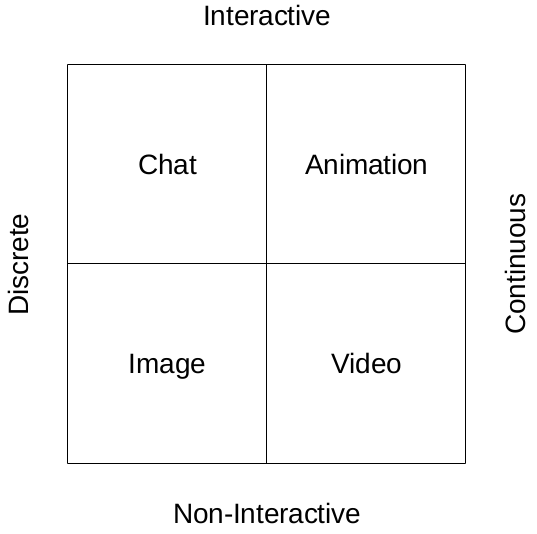
\includegraphics[width=0.35\textwidth]{figures/media_types.png}

	\caption{Media Types}
	\end{center}
\end{figure}

	Media Types can be described as discrete or continuos and interactive or non-interactive. For example an image is non-interctive and discrete, for instance, a video is continuos and non-interactive. A simple chat with just text is interactive and discrete. An animation that changes in function of user behaviour is interactive and continuous.

	Streaming protocols like \ac {RTP} were designed for continuous and non-interactive media types, such as audio and video. Discrete and non-interactive media don't need to streamed through \ac{RTP} because they don't change with. For example if an image appears in a specific time interval, just the \ac{HTML} or javascript that will reference the image must be streamed, the image itself is then transfered through \ac{HTTP}.

	In order to play any kind of stream, a player for interactive stream is needed downloading an environment, decoding the \ac{RTP} payload to determine the state and display it to the user. Streaming interactive media like the combination of \ac{HTML}, \ac{CSS} and JavaScript requires more than interpreting the code, a streamed user interface may contain an internal state that is not shown on code.

	Everytime an event is proccessed on one of the endpoints, both sender and receivers state must stay synchronized, otherwise events may behave differently.

	To achieve synchronization of interactive data most packets have three types: State, Delta-State and Event. State packet defines environment's complete state. Delta-State packets tranports just the piece of state that changed. Event packets informs that an event ocurred over the interactive media. 

	An \ac{RTP} recorder can have two operation modes, recording or playback. Traditional \ac{RTP} players can do random access, in contrast, interactive \ac{RTP} players must restore the environment and context at a given time. The environment is the initial state, so we can call it a non-interactive descrete media and handle it over \ac{HTTP}. After the receiver has received the environment, it should calculate the state at the given time. 

	If the \ac{RTP} recorder controls the correct data to send to the receivers, it cannot be a simple \ac{RTP} recorder as it must compute the state or delta-state to send. Therefore, if the receiver receives all recorded packets, it can calculate the current state from a nearest complete state. Having too much complete states, results on more precise random accesses but there is the storage space payback. On the other hand if there are few complete states recorded followed by delta-states, the recorded stream will occupy less storage space, but random accesses will be less granular.

	By recording and streaming the interactive media's complete state periodically, it is possible to restore the media state even if messages are lost.

	With such an interactive \ac{RTP} recorder it is then possible to record, play, fast forward, fast rewind, stop and jump to random positions.

  \cite{interactive_stream} proposed an \ac{RTP} profile for real-time transmission of interactive media. This new profile reuses much of video and audio profile implementation, integrating the interactive component.
	
  {\color{red}[Model View Controller (Suited for interactive RTP)]}


  {\color{red}[Identity]}



\quote{There is strong growth in the deployment of devices that integrate regular Web technologies such as HTML, CSS, and SVG, coupled with various device APIs.}

\subsection{Context}   % English
\subsection{Problem Statement / Solution Statement} % English
\subsection{Thesis Contributions} % English
\subsection{Article Structure} % English
% \section{Proposed Architecture} % English
\subsection{Methodology} % Section
\subsection{Planned Schedule} % English
\section{Conclusions} % English
\subsection{Summary} % English
\section{Conclusions} % English
\bibliographystyle{splncs03}
\bibliography{references}

\end{document}
